\section{Quantitative Results}
\subsection{NASA-TLX Results}
% TODO: position the table more near the bar graph
\begin{table}
    \centering
    \resizebox{\linewidth}{!}{
    \begin{tabular}{lccccc}
        \toprule
        % maybe add Raw TLX i.e summed up TLX
        Task & Mental Demand (Average) & Temporal Demand (Average) & Performance (Average) & Effort (Average) & Frustration (Average) \\
        \midrule
        Task 1 & 40.0 & 10.0 & 38.0 & 42.0 & 20.0 \\
        \midrule
        Task 2 & 24.0 & 10.0 & 37.0 & 35.0 & 10.0 \\
        \midrule
        Task 3 & 42.0 & 21.0 & 31.0 & 41.0 & 15.0 \\
        \midrule
        All Tasks combined & 35.3 & 13.7 & 35.3 & 39.3 & 15.0 \\
        \bottomrule
    \end{tabular}
    }
    \caption{Average NASA-TLX subscale scores per task}
    \label{tab:nasa-tlx-subscales-table}
\end{table}
\begin{figure}[h]
    \centering
    \definecolor{clrMental}{HTML}{4E79A7}
    \definecolor{clrTemporal}{HTML}{F28E2B}
    \definecolor{clrPerformance}{HTML}{59A14F}
    \definecolor{clrEffort}{HTML}{E15759}
    \definecolor{clrFrustration}{HTML}{B07AA1}
    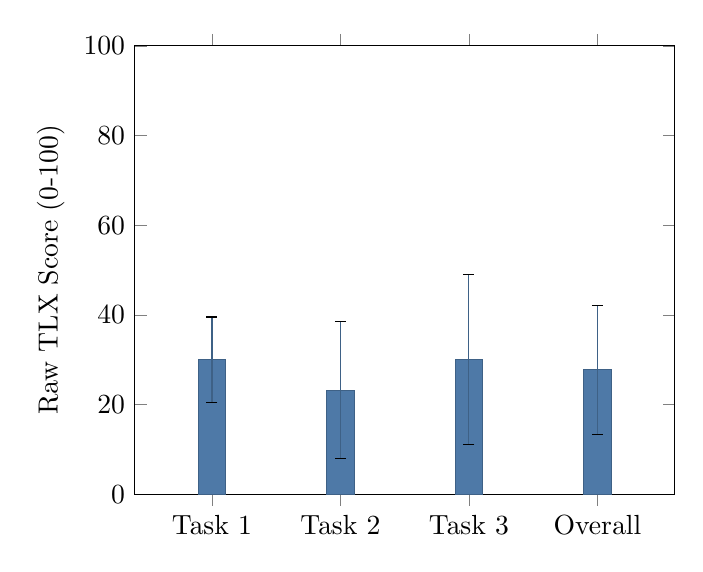
\begin{tikzpicture}
        \begin{axis}[
            ybar,
            compat=1.18,
            ylabel={Raw TLX Score (0-100)},
            ymin=0,
            ymax=100,
            symbolic x coords={Task 1, Task 2, Task 3, Overall},
            xtick=data,
            enlarge x limits=0.2,
            legend style={at={(0.5,-0.15)}, anchor=north, legend columns=-1},
            error bars/y dir=both,
            error bars/y explicit,
        ]
        % Mental Demand
        \addplot[fill=clrMental, draw=clrMental!80!black] coordinates {(Task 1, 30.0) +- (0, 9.5) (Task 2, 23.2) +- (0, 15.3) (Task 3, 30.0) +- (0, 18.9) (Overall, 27.7) +- (0, 14.4)};
        \end{axis}
    \end{tikzpicture}
    \caption{Raw TLX Scores for each Task and Average over all Tasks}
    \label{fig:raw-tlx-scores}
\end{figure}
The table \ref{tab:nasa-tlx-subscales-table} presents all the subscale means for each of the three tasks and overall. The figure \ref{fig:raw-tlx-scores} presents all the Raw TLX scores for the tasks and the overall Raw TLX score. The overall mean across all tasks is 27.7 (SD = 14.4). This indicates that the tool does not meaningfully overburden users when using it. Task 1 produced a mean Raw TLX score of 30.0 (SD = 9.5). In this task the Effort was the dominant subscale, with a mean score of 42.0. This can be explained that in this task, the user did not only had to understand but also correct a wrong VLOOKUP in the spreadsheet.
Task 2 produced the lowest mean Raw TLX score of the three tasks with a mean of 23.2 (SD = 15.3). Interesting is the subscale of perceived performance which has a mean of 37.0 but a standard deviation of 37.5 with values ranging from 5.0 up to 85.0. Which indicates that the participants had substantially different experiences of how well they accomplished the task, possibly reflecting genuine differences in accuracy or self-assessment. 
% Possibly assess how well participants did in certain questions and compare it to their self assessment.
Task 3 shared the same mean Raw TLX score as Task 1 but with a higher standard deviation of SD~=~18.9, possibly reflecting how multi-sheet spreadsheet have a stronger impact based on the individual. Interesting is that some Participants with low knowledge level like Participant 1 (Knowledge = 2) achieved a Raw TLX score of 12.0 while Participant 4 with a higher knowledge level (Knowledge = 6) achieved a substantial higher Raw TLX score of 39.0. The mean of the mental demand in Task 3 is 42.0 which is slightly higher than the one in Task 1 but not significantly higher. Which does not align with the assumption that multi-sheet spreadsheet have higher complexity than single sheet spreadsheets.
Across all tasks, Frustration was consistently the lowest-rated subscale with a mean of 15.0 (SD = 9.8). This indicates a positive signal, that even when participants encountered difficulties, they did not report sustained emotional frustration. 
%\begin{figure}[h]
    \centering
    \definecolor{clrMental}{HTML}{4E79A7}
    \definecolor{clrTemporal}{HTML}{F28E2B}
    \definecolor{clrPerformance}{HTML}{59A14F}
    \definecolor{clrEffort}{HTML}{E15759}
    \definecolor{clrFrustration}{HTML}{B07AA1}
    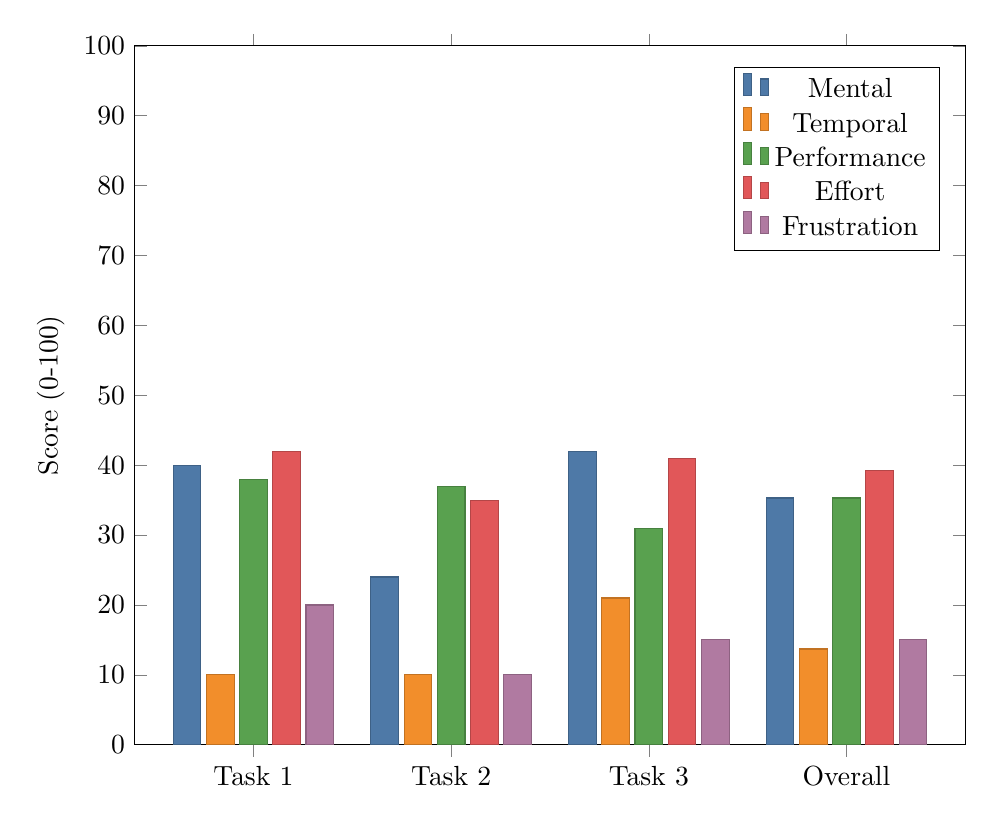
\begin{tikzpicture}
        \begin{axis}[
            ybar,
            compat=1.18,
            width=\linewidth,
            ylabel={Score (0-100)},
            ymin=0,
            ymax=100,
            symbolic x coords={Task 1, Task 2, Task 3, Overall},
            xtick=data,
            enlarge x limits=0.2,
            legend pos=north east,
        ]
        % Mental Demand
        \addplot[fill=clrMental, draw=clrMental!80!black] coordinates {(Task 1, 40.0) (Task 2, 24.0) (Task 3, 42.0) (Overall, 35.3)};
        % Temporal Demand
        \addplot[fill=clrTemporal, draw=clrTemporal!80!black] coordinates {(Task 1, 10.0) (Task 2, 10.0) (Task 3, 21.0) (Overall, 13.7)};
        % Performance
        \addplot[fill=clrPerformance, draw=clrPerformance!80!black] coordinates {(Task 1, 38.0) (Task 2, 37.0) (Task 3, 31.0) (Overall, 35.3)};
        % Effort
        \addplot[fill=clrEffort, draw=clrEffort!80!black] coordinates {(Task 1, 42.0) (Task 2, 35.0) (Task 3, 41.0) (Overall, 39.3)};
        % Frustration
        \addplot[fill=clrFrustration, draw=clrFrustration!80!black] coordinates {(Task 1, 20.0) (Task 2, 10.0) (Task 3, 15.0) (Overall, 15.0)};
        

        \legend{Mental, Temporal, Performance, Effort, Frustration}
        \end{axis}
    \end{tikzpicture}
    \caption{Subscale means for each task}
    \label{fig:tlx-task-subscales}
\end{figure}
\subsection{UEQ+ Results}
Figure \ref{fig:ueq-bar-graph} presents the means scores and standard deviations for each of the seven UEQ+-scales, alongside the mean importance and standard deviations provided by participants. All seven scales score above the neutral midpoint of 4, indicating that participants perceived the tool in general as positive. Efficiency (M = 5.95, SD = 0.84) and Clarity (M = 5.95, SD = 0.45) tie as the highest-rated scales. Which indicates that the participants had the impression, that the tool was helpful to solve the tasks without unnecessary effort. Important to mention is that Clarity exhibited the smallest standard deviation indicating a consensus that the tool was well organized and visually coherent. This consistency across participants with different expertise levels is a meaningful endorsement of the tool's architecture. The lowest score achieved the Dependability (M = 5.45, SD = 0.54), though it remained above the midpoint of 4.0. The lower scores appears connected to concerns about predictability and system supportiveness raised by individual participants. Especially Participant 4 rated the predictability and supportiveness at 4.0 while Participant 5, who has a comparable spreadsheet knowledge, rated it 7.0 and 6.0. 
When comparing the scale scores with their importance ratings, perspicuity, the scale capturing how understandable and learnable the tool is, received the highest importance rating of all scales (M = 6.40, SD = 0.55). This indicates that learnability is the quality the participants most care about in this tool. The tool delievered on this dimension according to the participant, because the score of Perspicuity is 5.75. Visual Aesthetics received the most polarised importance rating ranging (M = 4.60, SD = 1.82). For some participants the aesthetics were extremely important, indicated with a score of 7/7, and for other users it was almost irrelevant, indicated with a score of 3/7. This suggests that aesthetic refinement is not a priority for this tool.
The importance ratings further reveal a hierarchy of user priorities. Usefulness and Perspicuity tied as the most important qualities (both M = 6.20 and M = 6.40 respectively). Structure and Visual Aesthetics received the lowest importance ratings (M = 5.20 and M = 4.60), suggesting that while these dimensions are pleasant, that it is more important if the tool can help them understand the spreadsheet.
\begin{figure}[h]
    \centering
    \definecolor{clrMental}{HTML}{4E79A7}
    \definecolor{clrTemporal}{HTML}{F28E2B}
    \definecolor{clrPerformance}{HTML}{59A14F}
    \definecolor{clrEffort}{HTML}{E15759}
    \definecolor{clrFrustration}{HTML}{B07AA1}
    \resizebox{\linewidth}{!}{%
    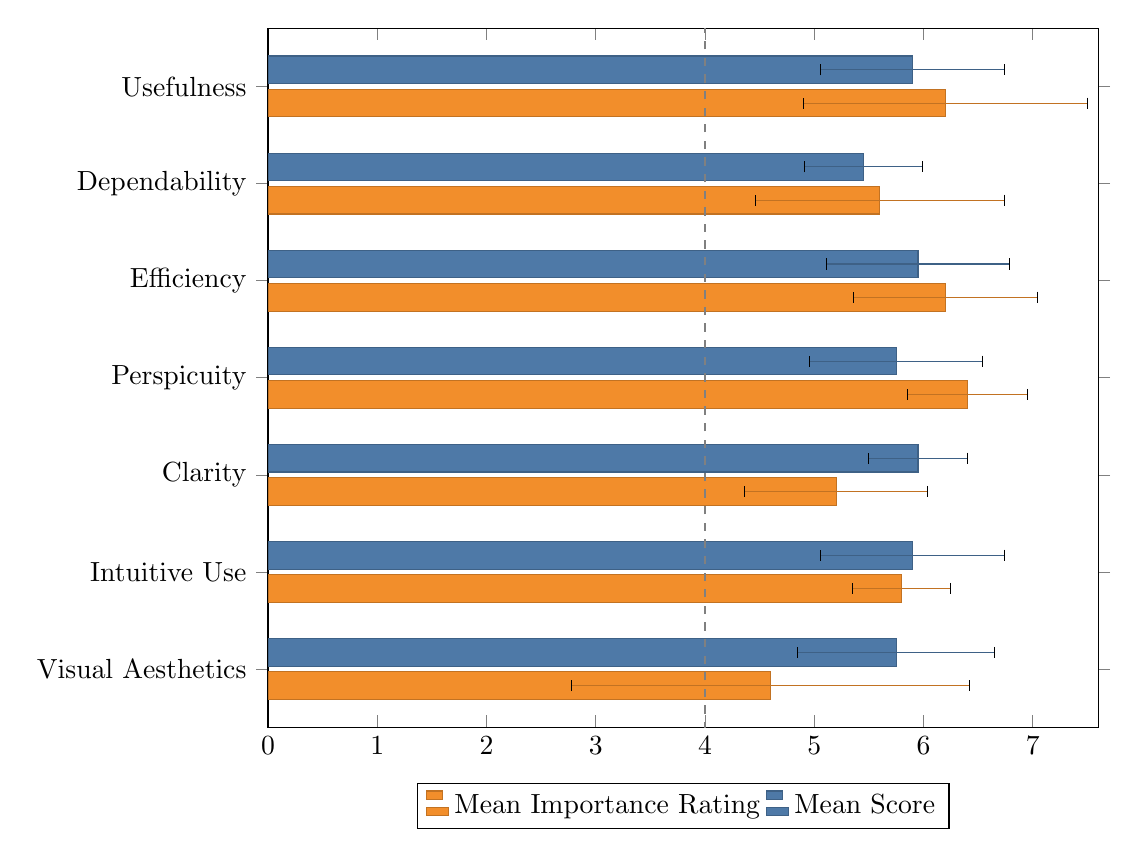
\begin{tikzpicture}
        \begin{axis}[
            xbar,
            ytick={1,...,7},
            yticklabels={Visual Aesthetics, Intuitive Use, Clarity, Perspicuity, Efficiency, Dependability, Usefulness},
            width=\linewidth,
            xmin=0,
            xmax=7.6,
            xtick={0,1,2,3,4,5,6,7},
            enlarge y limits=0.1,
            legend style={
                at={(0.5,-0.08)},
                anchor=north,
                legend columns=-1,
            },
        ]
        % y=1 Visual Aesthetics, y=2 Intuitive Use, y=3 Structure, y=4 Perspicuity,
        % y=5 Efficiency, y=6 Dependability, y=7 Usefulness
        % Scale importances
        \addplot[
            fill=clrTemporal, draw=clrTemporal!80!black,
            error bars/.cd, x dir=both, x explicit,
        ] coordinates {
            (4.60,1) +- (1.82,0)
            (5.80,2) +- (0.45,0)
            (5.20,3) +- (0.84,0)
            (6.40,4) +- (0.55,0)
            (6.20,5) +- (0.84,0)
            (5.60,6) +- (1.14,0)
            (6.20,7) +- (1.30,0)
        };
        % Scale ratings
        \addplot[
            fill=clrMental, draw=clrMental!80!black,
            error bars/.cd, x dir=both, x explicit,
        ] coordinates {
            (5.75,1) +- (0.90,0)
            (5.90,2) +- (0.84,0)
            (5.95,3) +- (0.45,0)
            (5.75,4) +- (0.79,0)
            (5.95,5) +- (0.84,0)
            (5.45,6) +- (0.54,0)
            (5.90,7) +- (0.84,0)
        };

        \draw[dashed, gray] (axis cs:4,-1) -- (axis cs:4,10);

        \legend{Mean Importance Rating, Mean Score}
        \end{axis}
    \end{tikzpicture}}%
    \caption{Mean scores of the UEQ+ sclaes}
    \label{fig:ueq-bar-graph}
\end{figure}